\documentclass{article}%
\usepackage[T1]{fontenc}%
\usepackage[utf8]{inputenc}%
\usepackage{lmodern}%
\usepackage{textcomp}%
\usepackage{lastpage}%
\usepackage{parskip}%
\usepackage[top=1.2in,bottom=1in,left=0.6in,right=0.6in,headsep=0.8in]{geometry}%
\usepackage{amsmath}%
\usepackage{graphicx}%
\usepackage{needspace}%
\usepackage{color}%
\usepackage{longtable}%
\usepackage{multirow}%
\usepackage[table]{xcolor}%
\usepackage{fancyhdr}%
\usepackage{tabularx}%
%
\definecolor{OsdagGreen}{HTML}{D5DF93}%
\fancypagestyle{header}{ 
\renewcommand{\headrulewidth}{0pt}%
\renewcommand{\footrulewidth}{0pt}%
\fancyhead{ 
}%
\fancyfoot{ 
}%
\fancyhead[C]{ 
\begin{tabularx}{\textwidth}{|l|p{6cm}|l|X|}%
\hline%
\rowcolor{OsdagGreen}%
Company Name&LoremIpsum&Project Title&Fossee\\%
\hline%
\rowcolor{OsdagGreen}%
Group/Team Name&LoremIpsum&Subtitle&\\%
\hline%
\rowcolor{OsdagGreen}%
Designer&LoremIpsum&Job Number&123\\%
\hline%
\rowcolor{OsdagGreen}%
Date&26 /05 /2020&Client&LoremIpsum\\%
\hline%
\end{tabularx}
}%
\fancyfoot[R]{ 
Page \thepage\ of \pageref{LastPage}
}
}%
%
\begin{document}%
\normalsize%
\pagestyle{header}%
\section{Input Parameters}%
\label{sec:InputParameters}%
\renewcommand{\arraystretch}{1.2}%
\begin{longtable}{|p{5cm}|p{2cm}|p{2cm}|p{2cm}|p{5cm}|}%
\hline%
\hline%
\multicolumn{3}{|c|}{Module}&\multicolumn{2}{|c|}{Beam Coverplate Connection}\\%
\hline%
\hline%
\multicolumn{3}{|c|}{MainModule}&\multicolumn{2}{|c|}{Moment Connection}\\%
\hline%
\hline%
\multicolumn{3}{|c|}{Moment(kNm)*}&\multicolumn{2}{|c|}{50.0}\\%
\hline%
\hline%
\multicolumn{3}{|c|}{Shear (kN)*}&\multicolumn{2}{|c|}{50.0}\\%
\hline%
\hline%
\multicolumn{3}{|c|}{Axial (kN) *}&\multicolumn{2}{|c|}{30.0}\\%
\hline%
\hline%
\multicolumn{5}{|c|}{\textbf{Section}}\\%
\hline%
\hline%
\multirow{12}{*}{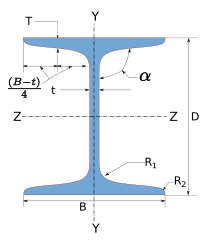
\includegraphics[width=5cm,height=5cm]{E:/office _anjali/columnspliceanjali/Osdag3/ResourceFiles/images/ISection.png}}&\multicolumn{2}{|c|}{Beam Section *}&\multicolumn{2}{|c|}{NPB 600x220x122.4}\\%
\cline{2%
-%
5}%
&\multicolumn{2}{|c|}{Preferences}&\multicolumn{2}{|c|}{Outside}\\%
\cline{2%
-%
5}%
&\multicolumn{2}{|c|}{Material *}&\multicolumn{2}{|c|}{E 250 (Fe 410 W)A}\\%
\cline{2%
-%
5}%
&\multicolumn{2}{|c|}{Ultimate strength, fu (MPa)}&\multicolumn{2}{|c|}{410}\\%
\cline{2%
-%
5}%
&Yield Strength , fy (MPa)&250&R1(mm)&2.4\\%
\cline{2%
-%
5}%
&Mass&122.45&R2(mm)&0.0\\%
\cline{2%
-%
5}%
&Area(mm2) {-} A&15600.0&Iz(mm4)&920834000.0\\%
\cline{2%
-%
5}%
&D(mm)&600.0&Iy(mm4)&33828700.0\\%
\cline{2%
-%
5}%
&B(mm)&220.0&rz(mm)&243.0\\%
\cline{2%
-%
5}%
&t(mm)&12.0&ry(mm)&46.6\\%
\cline{2%
-%
5}%
&T(mm)&19.0&Zz(mm3)&3069450.0\\%
\cline{2%
-%
5}%
&FlangeSlope&90&Zy(mm3)&307530.0\\%
\cline{2%
-%
5}%
\hline%
\multicolumn{5}{|c|}{\textbf{Bolt Details}}\\%
\hline%
\hline%
\multicolumn{3}{|c|}{Diameter (mm)*}&\multicolumn{2}{|c|}{{[}12.0, 16.0, 20.0, 24.0, 30.0, 36.0{]}}\\%
\hline%
\hline%
\multicolumn{3}{|c|}{Grade *}&\multicolumn{2}{|c|}{{[}3.6, 4.6, 4.8, 5.6, 5.8, 6.8, 8.8, 9.8, 10.9, 12.9{]}}\\%
\hline%
\hline%
\multicolumn{3}{|c|}{Type *}&\multicolumn{2}{|c|}{Bearing Bolt}\\%
\hline%
\hline%
\multicolumn{3}{|c|}{Bolt hole type}&\multicolumn{2}{|c|}{Standard}\\%
\hline%
\hline%
\multicolumn{3}{|c|}{Slip factor (µ\_f)}&\multicolumn{2}{|c|}{0.3}\\%
\hline%
\hline%
\multicolumn{3}{|c|}{Type of edges}&\multicolumn{2}{|c|}{a {-} Sheared or hand flame cut}\\%
\hline%
\hline%
\multicolumn{3}{|c|}{Gap between beam and <br>support (mm)}&\multicolumn{2}{|c|}{10.0}\\%
\hline%
\hline%
\multicolumn{3}{|c|}{Are the members exposed to <br>corrosive influences}&\multicolumn{2}{|c|}{False}\\%
\hline%
\end{longtable}

%
\Needspace{10\baselineskip}%
\newpage%
\section{Design Checks}%
\label{sec:DesignChecks}%
\subsection{Member Capacity}%
\label{subsec:MemberCapacity}%
\renewcommand{\arraystretch}{1.2}%
\begin{longtable}{|p{4cm}|p{5cm}|p{5.5cm}|p{1.5cm}|}%
\hline%
\rowcolor{OsdagGreen}%
Check&Required&Provided&Remarks\\%
\hline%
\endhead%
\hline%
Axial Capacity Member Ac (kN)&&$\begin{aligned} A_c &=\frac{A*f_y}{\gamma_{m0} *10^3}\\ &=\frac{15600.0*250}{1.1* 10^3}\\ &=3545.45\end{aligned}$&\\%
\hline%
Shear Capacity Member Sc (kN)&&$\begin{aligned} S_c &= \frac{A_v*f_y}{\sqrt{3}*\gamma_{mo} *10^3}\\ &=\frac{562.0*12.0*250}{\sqrt{3}*1.1 *10^3}\\ &=884.92\end{aligned}$&\\%
\hline%
Plastic Moment Capacity Pmc (kNm)&&$\begin{aligned} Pmc &= \frac{\beta_b * Z_p *fy}{\gamma_{mo} * 10^6}\\ &=\frac{1*947532.0*250}{1.1 * 10^6}\\ &=215.35\end{aligned}$&\\%
\hline%
Moment Deformation Criteria Mdc (kNm)&&$\begin{aligned} Mdc &= \frac{1.5 *Z_e *fy}{1.1* 10^6}\\ &= \frac{1.5 *3069450.0*250}{1.1* 10^6}\\ &= 1046.4\end{aligned}$&\\%
\hline%
Moment Capacity Member Mc (kNm)&&$\begin{aligned} M_c &= min(Pmc,Mdc)\\ &=min(215.35,1046.4)\\ &=215.35\end{aligned}$&\\%
\hline%
\end{longtable}

%
\newpage%
\subsection{Load Consideration}%
\label{subsec:LoadConsideration}%
\renewcommand{\arraystretch}{1.2}%
\begin{longtable}{|p{4cm}|p{3.5cm}|p{6.5cm}|p{1.5cm}|}%
\hline%
\rowcolor{OsdagGreen}%
Check&Required&Provided&Remarks\\%
\hline%
\endhead%
\hline%
Applied Axial Load Au (kN)&$\begin{aligned} Ac_{min} &= 0.3 * A_c\\ &= 0.3 *3545.45\\ &=1063.64\\ Ac_{max} &= Ac \\ &=3545.45\end{aligned}$&$\begin{aligned} A_u &=1063.64\end{aligned}$&Pass\\%
\hline%
Applied Shear Load Vu (kN)&$\begin{aligned} Vc_{min} &= 0.6 * S_c\\ &= 0.6 *884.92\\ &=530.95\\ Vc_{max} &= Sc \\ &=884.92\end{aligned}$&$\begin{aligned} V_u &=530.95\end{aligned}$&Pass\\%
\hline%
Applied Moment Load Mu (kNm)&$\begin{aligned} Mc_{min} &= 0.5 * M_c\\ &= 0.5 *215.35\\ &=107.67\\  Mc_{max} &= Mc \\ &=215.35\end{aligned}$&$\begin{aligned} M_u &=107.67\end{aligned}$&Pass\\%
\hline%
Forces Carried by Web&&$\begin{aligned}A_w &= Axial~ force~ in~ web  \\   &= \frac{(D- 2*T)*t* Au }{A} \\ &= \frac{(600.0- 2*19.0)*12.0*1063.64 }{15600.0} \\ &=459.82~ kN\\ M_w &= Moment ~in ~web  \\  &= \frac{Z_w * Mu}{Z} \\ &= \frac{947532.0 * 107.67}{3512400.0} \\ &=29.05~{kNm}\end{aligned}$&\\%
\hline%
Forces Carried by Flange&&$\begin{aligned} A_f&= Axial~force~ in ~flange  \\ &= \frac{Au * B *T}{A} \\ &= \frac{1063.64 * 220.0*19.0}{15600.0} \\ &=285.0~ kN\\ M_f& =Moment~ in~ flange \\  & = Mu-M_w\\ &= 107.67-29.05\\ &=78.63~{kNm}\\  F_f& =flange~force  \\ & = \frac{M_f *10^3}{D-T} + A_f \\ &= \frac{78.63* 10^3}{600.0-19.0} +285.0 \\ &=420.33~kN \end{aligned}$&\\%
\hline%
\end{longtable}

%
\newpage%
\subsection{Initial Member Check}%
\label{subsec:InitialMemberCheck}%
\renewcommand{\arraystretch}{1.2}%
\begin{longtable}{|p{3cm}|p{4.5cm}|p{6.5cm}|p{1.5cm}|}%
\hline%
\rowcolor{OsdagGreen}%
Check&Required&Provided&Remarks\\%
\hline%
\endhead%
\hline%
Flange Tension Yielding Capacity (kN)&$\begin{aligned} F_f &=420.33\end{aligned}$&$\begin{aligned} T_{dg} &= \frac{l*t*f_y}{\gamma_{mo}}\\ &=\frac{1*220.0*19.0*250}{1.1}\\ &=950.0\end{aligned}$&Pass\\%
\hline%
Web Tension Yielding Capacity (kN)&$\begin{aligned} A_w &=459.82\end{aligned}$&$\begin{aligned} T_{dg} &= \frac{l*t*f_y}{\gamma_{mo}}\\ &=\frac{1*562.0*12.0*250}{1.1}\\ &=1533\end{aligned}$&Pass\\%
\hline%
\end{longtable}

%
\newpage%
\subsection{Initial flange plate height check}%
\label{subsec:Initialflangeplateheightcheck}%
\renewcommand{\arraystretch}{1.2}%
\begin{longtable}{|p{4.5cm}|p{2.5cm}|p{7cm}|p{1.5cm}|}%
\hline%
\rowcolor{OsdagGreen}%
Check&Required&Provided&Remarks\\%
\hline%
\endhead%
\hline%
flange\_plate.Height&Outer.b >= 50&$\begin{aligned} Outer.b &=220.0\end{aligned}$&Pass\\%
\hline%
\end{longtable}

%
\newpage%
\subsection{Flange plate thickness}%
\label{subsec:Flangeplatethickness}%
\renewcommand{\arraystretch}{1.2}%
\begin{longtable}{|p{2.5cm}|p{4.5cm}|p{7cm}|p{1.5cm}|}%
\hline%
\rowcolor{OsdagGreen}%
Check&Required&Provided&Remarks\\%
\hline%
\endhead%
\hline%
Thickness (mm)*&$\begin{aligned} T &=19.0\end{aligned}$&$\begin{aligned} t_f &=20.0\end{aligned}$&Pass\\%
\hline%
Plate Area check (mm2)&$\begin{aligned} &pt.area >= \\&connected~member~area * 1.05\\  &= 4389.0\end{aligned}$&$\begin{aligned} outer.b &= B\\ &= 220.0\\  pt.area &= 20.0 * 220.0\\ &= 4400.0\end{aligned}$&Pass\\%
\hline%
\end{longtable}

%
\newpage%
\subsection{Web plate thickness}%
\label{subsec:Webplatethickness}%
\renewcommand{\arraystretch}{1.2}%
\begin{longtable}{|p{2.5cm}|p{4.5cm}|p{7cm}|p{1.5cm}|}%
\hline%
\rowcolor{OsdagGreen}%
Check&Required&Provided&Remarks\\%
\hline%
\endhead%
\hline%
Thickness (mm)*&$\begin{aligned} t &=6.0\end{aligned}$&$\begin{aligned} t_w &=8.0\end{aligned}$&Pass\\%
\hline%
Plate Area check (mm2)&$\begin{aligned} &pt.area >= \\&connected~member~area * 1.05\\  &= 6325.2\end{aligned}$&$\begin{aligned} web~b &= D-(2*T)-(2*r_1)\\ &=600.0-(2*19.0)-(2*2.4)\\ &= 502.0 \\  pt.area &= 8.0*2* 502.0\\ &= 8032.0\end{aligned}$&Pass\\%
\hline%
\end{longtable}

%
\newpage%
\subsection{Web Spacing Checks}%
\label{subsec:WebSpacingChecks}%
\renewcommand{\arraystretch}{1.2}%
\begin{longtable}{|p{2.5cm}|p{7.5cm}|p{5cm}|p{1cm}|}%
\hline%
\rowcolor{OsdagGreen}%
Check&Required&Provided&Remarks\\%
\hline%
\endhead%
\hline%
Min.Diameter (mm)&&$\begin{aligned} d &=12.0\end{aligned}$&\\%
\hline%
Min. Gauge (mm)&$\begin{aligned}p/g_{min}&= 2.5 ~ d&\\ =&2.5*12.0&=30.0\end{aligned}$&$\begin{aligned} g &=50~(Row~Limit~(r_l) = 2)\end{aligned}$&\\%
\hline%
Min. Edge Distance (mm)&$\begin{aligned}e/e`_{min} &=[1.5~or~ 1.7] * d_0\\ &=1.7*13.0=22.1 \end{aligned}$&40&\\%
\hline%
Spacing Check&$\begin{aligned} depth & = 2 * e + (r_l -1) * g\\ & = 2 * 40+(2.0-1)*50\\ & = 130.0\end{aligned}$&502.0&Pass\\%
\hline%
\end{longtable}

%
\newpage%
\subsection{Flange Spacing Checks}%
\label{subsec:FlangeSpacingChecks}%
\renewcommand{\arraystretch}{1.2}%
\begin{longtable}{|p{2.5cm}|p{7.5cm}|p{5cm}|p{1cm}|}%
\hline%
\rowcolor{OsdagGreen}%
Check&Required&Provided&Remarks\\%
\hline%
\endhead%
\hline%
Min.Diameter (mm)&&$\begin{aligned} d &=12.0\end{aligned}$&\\%
\hline%
Min. Gauge (mm)&$\begin{aligned}p/g_{min}&= 2.5 ~ d&\\ =&2.5*12.0&=30.0\end{aligned}$&$\begin{aligned} g &=0.0~(Row~Limit~(r_l) = 1)\end{aligned}$&\\%
\hline%
Min. Edge Distance (mm)&$\begin{aligned}e/e`_{min} &=[1.5~or~ 1.7] * d_0\\ &=1.7*13.0=22.1 \end{aligned}$&40&\\%
\hline%
Spacing Check&$\begin{aligned} depth & = 2 * e + (r_l -1) * g\\ & = 2 * 40+(1.0-1)*50\\ & = 80.0\end{aligned}$&101.6&Pass\\%
\hline%
\end{longtable}

%
\newpage%
\subsection{Flange Bolt Checks}%
\label{subsec:FlangeBoltChecks}%
\renewcommand{\arraystretch}{1.2}%
\begin{longtable}{|p{4cm}|p{5cm}|p{5.5cm}|p{1.5cm}|}%
\hline%
\rowcolor{OsdagGreen}%
Check&Required&Provided&Remarks\\%
\hline%
\endhead%
\hline%
Diameter (mm)&Bolt Quantity Optimisation&$\begin{aligned} d &=20.0\end{aligned}$&\\%
\hline%
Grade&Bolt Grade Optimisation&10.9&\\%
\hline%
Bolt.fu&&1000.0&\\%
\hline%
Bolt.fy&&900.0&\\%
\hline%
Hole Diameter (mm)& &$\begin{aligned} d_0 &=22.0\end{aligned}$&\\%
\hline%
Shear Capacity (kN)&&$\begin{aligned}V_{dsb} &= \frac{f_{ub} ~n_n~ A_{nb}}{\sqrt{3} ~\gamma_{mb}}\\ &= \frac{1000.0*1*245}{\sqrt{3}~*~1.25}\\ &= 113.16\end{aligned}$&\\%
\hline%
Bearing Capacity (kN)&&$\begin{aligned}V_{dpb} &= \frac{2.5~ k_b~ d~ t~ f_u}{\gamma_{mb}}\\ &= \frac{2.5~*0.51*20.0*19.0*410}{1.25}\\ &=158.92\end{aligned}$&\\%
\hline%
Bolt Capacity (kN)&&$\begin{aligned}V_{db} &= min~ (V_{dsb}, V_{dpb})\\ &= min~ (113.16,158.92)\\ &=113.16\end{aligned}$&\\%
\hline%
No of Bolts&$\begin{aligned}R_{u} &= \sqrt{V_u^2+A_u^2}\\ n_{trial} &= R_u/ V_{bolt}\\ R_{u} &= \frac{\sqrt{0.0^2+420.33^2}}{113.16}\\ &=8\end{aligned}$&8&\\%
\hline%
No of Columns&&$\begin{aligned} n_c &=4\end{aligned}$&\\%
\hline%
No of Rows&&$\begin{aligned} n_r &=2\end{aligned}$&\\%
\hline%
Min. Pitch (mm)&$\begin{aligned}p/g_{min}&= 2.5 ~ d&\\ =&2.5*20.0&=50.0\end{aligned}$&50&Pass\\%
\hline%
Max. Pitch (mm)&$\begin{aligned}p/g_{max} &=\min(32~t,~300~mm)&\\ &=\min(32 *~19.0,~ 300 ~mm)\\&=300\end{aligned}$&50&Pass\\%
\hline%
Min. Gauge (mm)&$\begin{aligned}p/g_{min}&= 2.5 ~ d&\\ =&2.5*20.0&=50.0\end{aligned}$&0.0&N/A\\%
\hline%
Max. Gauge (mm)&$\begin{aligned}p/g_{max} &=\min(32~t,~300~mm)&\\ &=\min(32 *~19.0,~ 300 ~mm)\\&=300\end{aligned}$&0.0&N/A\\%
\hline%
Min. End Distance (mm)&$\begin{aligned}e/e`_{min} &=[1.5~or~ 1.7] * d_0\\ &=1.7*22.0=37.4 \end{aligned}$&40&Pass\\%
\hline%
Max. End Distance (mm)&$\begin{aligned}e/e`_{max} &= 12~ t~ \varepsilon&\\ \varepsilon &= \sqrt{\frac{250}{f_y}}\\ e/e`_{max}&=12 ~*20.0*\sqrt{\frac{250}{250}}\\ &=240.0\\ \end{aligned}$&40&Pass\\%
\hline%
Min. Edge Distance (mm)&$\begin{aligned}e/e`_{min} &=[1.5~or~ 1.7] * d_0\\ &=1.7*22.0=37.4 \end{aligned}$&50.8&Pass\\%
\hline%
Max. Edge Distance (mm)&$\begin{aligned}e/e`_{max} &= 12~ t~ \varepsilon&\\ \varepsilon &= \sqrt{\frac{250}{f_y}}\\ e/e`_{max}&=12 ~*20.0*\sqrt{\frac{250}{250}}\\ &=240.0\\ \end{aligned}$&50.8&Pass\\%
\hline%
Bolt Capacity post Long Joint (kN)&$\begin{aligned} &if~l\geq 15 * d~then~V_{rd} = \beta_{ij} * V_{db} \\ & if~l < 15 * d~then~V_{rd} = V_{db} \\ & where,\\ & l = ((nc~or~nr) - 1) * (p~or~g) \\ & \beta_{ij} = 1.075 - l/(200 * d) \\ & but~0.75\leq\beta_{ij}\leq1.0 \end{aligned}$&$\begin{aligned} l~&= ((nc~or~nr) - 1) * (p~or~g) \\  lc&= 2*((\frac{4}{2} - 1) * 50+40)+ 10.0\\&=190.0\\  lr&= 2*((\frac{2}{2} - 1) * 0.0+50.8\\& +2.4)+ 12.0=118.39999999999999\\  l~&= 190.0\\ & 15 * d = 15 * 20.0 = 300.0 \\ & since,~l < 15 * d~ \\& then~V_{rd} = V_{db} \\ & V_{rd} = 113.16 \end{aligned}$&\\%
\hline%
Capacity (kN)&105.08&113.16&Pass\\%
\hline%
\end{longtable}

%
\newpage%
\subsection{Web Bolt Checks}%
\label{subsec:WebBoltChecks}%
\renewcommand{\arraystretch}{1.2}%
\begin{longtable}{|p{4cm}|p{5cm}|p{5.5cm}|p{1.5cm}|}%
\hline%
\rowcolor{OsdagGreen}%
Check&Required&Provided&Remarks\\%
\hline%
\endhead%
\hline%
Shear Capacity (kN)&&$\begin{aligned}V_{dsb} &= \frac{f_{ub} ~n_n~ A_{nb}}{\sqrt{3} ~\gamma_{mb}}\\ &= \frac{1000.0*2*245}{\sqrt{3}~*~1.25}\\ &= 226.32\end{aligned}$&\\%
\hline%
Bearing Capacity (kN)&&$\begin{aligned}V_{dpb} &= \frac{2.5~ k_b~ d~ t~ f_u}{\gamma_{mb}}\\ &= \frac{2.5~*0.51*20.0*12.0*410}{1.25}\\ &=100.37\end{aligned}$&\\%
\hline%
Bolt Capacity (kN)&&$\begin{aligned}V_{db} &= min~ (V_{dsb}, V_{dpb})\\ &= min~ (226.32,100.37)\\ &=100.37\end{aligned}$&\\%
\hline%
No of Bolts&$\begin{aligned}R_{u} &= \sqrt{V_u^2+A_u^2}\\ n_{trial} &= R_u/ V_{bolt}\\ R_{u} &= \frac{\sqrt{530.95^2+459.82^2}}{100.37}\\ &=14\end{aligned}$&28&\\%
\hline%
No of Columns&&$\begin{aligned} n_c &=4\end{aligned}$&\\%
\hline%
No of Rows&&$\begin{aligned} n_r &=7\end{aligned}$&\\%
\hline%
Min. Pitch (mm)&$\begin{aligned}p/g_{min}&= 2.5 ~ d&\\ =&2.5*20.0&=50.0\end{aligned}$&50&Pass\\%
\hline%
Max. Pitch (mm)&$\begin{aligned}p/g_{max} &=\min(32~t,~300~mm)&\\ &=\min(32 *~8.0,~ 300 ~mm)\\&=256.0\end{aligned}$&50&Pass\\%
\hline%
Min. Gauge (mm)&$\begin{aligned}p/g_{min}&= 2.5 ~ d&\\ =&2.5*20.0&=50.0\end{aligned}$&65&Pass\\%
\hline%
Max. Gauge (mm)&$\begin{aligned}p/g_{max} &=\min(32~t,~300~mm)&\\ &=\min(32 *~8.0,~ 300 ~mm)\\&=256.0\end{aligned}$&65&Pass\\%
\hline%
Min. End Distance (mm)&$\begin{aligned}e/e`_{min} &=[1.5~or~ 1.7] * d_0\\ &=1.7*22.0=37.4 \end{aligned}$&40&Pass\\%
\hline%
Max. End Distance (mm)&$\begin{aligned}e/e`_{max} &= 12~ t~ \varepsilon&\\ \varepsilon &= \sqrt{\frac{250}{f_y}}\\ e/e`_{max}&=12 ~*8.0*\sqrt{\frac{250}{250}}\\ &=96.0\\ \end{aligned}$&40&Pass\\%
\hline%
Min. Edge Distance (mm)&$\begin{aligned}e/e`_{min} &=[1.5~or~ 1.7] * d_0\\ &=1.7*22.0=37.4 \end{aligned}$&40&Pass\\%
\hline%
Max. Edge Distance (mm)&$\begin{aligned}e/e`_{max} &= 12~ t~ \varepsilon&\\ \varepsilon &= \sqrt{\frac{250}{f_y}}\\ e/e`_{max}&=12 ~*8.0*\sqrt{\frac{250}{250}}\\ &=96.0\\ \end{aligned}$&40&Pass\\%
\hline%
Parameters required for bolt force (mm)&&$\begin{aligned} l_n~~~ &= length~available \\  l_n~~~ &= (n_r - 1) * g\\  &= (7 - 1) *65\\  & =390\\  y_{max} &= l_n / 2\\  &= 390 / 2 \\  & =195.0\\ x_{max} &= p * (\frac{n_c}{2} - 1) / 2 \\  &= 50 * (\frac{4}{2} + - 1) / 2 \\  & =25.0\end{aligned}$&\\%
\hline%
Moment Demand (kNm&&$\begin{aligned}  M_d &= (V_u * ecc + M_w)\\  &= \frac{(530.95 * 10^3 *70.0 + 29.05*10^6)}{10^6}\\  & =66.21\end{aligned}$&\\%
\hline%
Bolt.Force&&$\begin{aligned} vbv~~ &= V_u / (n_r * n_c)\\  &= \frac{530.95}{ (7*4)}\\  & =37.93\\ tmh~ &= \frac{M_d * y_{max} }{ \Sigma r_i^2} \\  &= \frac{66.21 *195.0}{245.35}\\  & =52.63\\  tmv ~&= \frac{M_d * x_{max}}{\Sigma r_i^2}\\ &= \frac{66.21 * 25.0}{245.35}\\  & =6.75\\  abh~ & = \frac{A_u }{(n_r * n_c)}\\   & =\frac{459.82}{ (7 *4)}\\  & =32.84\\  vres &=\sqrt{(vbv +tmv) ^ 2 + (tmh+abh) ^ 2}\\   &= \sqrt{(37.93 +6.75) ^2 + (52.63+32.84) ^ 2}\\  & =96.44\end{aligned}$&\\%
\hline%
Bolt Capacity post Long Joint (kN)&$\begin{aligned} &if~l\geq 15 * d~then~V_{rd} = \beta_{ij} * V_{db} \\ & if~l < 15 * d~then~V_{rd} = V_{db} \\ & where,\\ & l = ((nc~or~nr) - 1) * (p~or~g) \\ & \beta_{ij} = 1.075 - l/(200 * d) \\ & but~0.75\leq\beta_{ij}\leq1.0 \end{aligned}$&$\begin{aligned} l&= ((nc~or~nr) - 1) * (p~or~g) \\  lc&= 2*((\frac{4}{2} - 1) * 50+40)+ 10.0\\&=190.0\\  lr&= (7 - 1) * 65=390\\  l&= 390\\ & 15 * d = 15 * 20.0 = 300.0 \\ &since,~l \geq 15 * d~ \\&then~V_{rd} = \beta_{ij} * V_{db} \\ \beta_{ij} &= 1.075 - 390/(200*20.0) \\&=0.98\\ V_{rd} &= 0.98 * 100.37=98.36 \end{aligned}$&\\%
\hline%
Capacity (kN)&96.44&98.36&Pass\\%
\hline%
\end{longtable}

%
\newpage%
\subsection{Outer flange plate Checks}%
\label{subsec:OuterflangeplateChecks}%
\renewcommand{\arraystretch}{1.2}%
\begin{longtable}{|p{4cm}|p{6cm}|p{5.5cm}|p{1.5cm}|}%
\hline%
\rowcolor{OsdagGreen}%
Check&Required&Provided&Remarks\\%
\hline%
\endhead%
\hline%
Min. Plate Height (mm)&$\begin{aligned}min~flange~plate~ht &= beam~width\\ &=220.0\end{aligned}$&220.0&Pass\\%
\hline%
Min. Plate Length (mm)&$\begin{aligned} & 2[2*e_{min} + ({\frac{bolt~lines}{2}}-1) * p_{min})]\\ & +\frac{gap}{2}]\\ &=2*[(2*37.4 + (\frac{4}{2}-1) * 50.0\\ &= + \frac{10.0}{2}]\\ &=259.6\end{aligned}$&270.0&Pass\\%
\hline%
Min.Plate Thickness (mm)&$\begin{aligned} t_w=19.0\end{aligned}$&20.0&Pass\\%
\hline%
\end{longtable}

%
\newpage%
\subsection{Member Checks}%
\label{subsec:MemberChecks}%
\renewcommand{\arraystretch}{1.2}%
\begin{longtable}{|p{4cm}|p{6cm}|p{5.5cm}|p{1.5cm}|}%
\hline%
\rowcolor{OsdagGreen}%
Check&Required&Provided&Remarks\\%
\hline%
\endhead%
\hline%
Flange Tension Yielding Capacity (kN)&&$\begin{aligned} T_{dg} &= \frac{l*t*f_y}{\gamma_{mo}}\\ &=\frac{1*220.0*19.0*250}{1.1}\\ &=950.0\end{aligned}$&\\%
\hline%
Flange Tension Rupture Capacity (kN)&&$\begin{aligned} T_{dn} &= \frac{0.9*A_{n}*f_u}{\gamma_{m1}}\\ &=\frac{0.9*(220.0-2*22.0)*19.0*410}{1.25}\\ &=987.15\end{aligned}$&\\%
\hline%
Flange Block Shear Capacity (kN)&&$\begin{aligned}T_{db1} &= \frac{A_{vg} f_{y}}{\sqrt{3} \gamma_{m0}} + \frac{0.9 A_{tn} f_{u}}{\gamma_{m1}}\\ T_{db2} &= \frac{0.9*A_{vn} f_{u}}{\sqrt{3} \gamma_{m1}} + \frac{A_{tg} f_{y}}{\gamma_{m0}}\\ T_{db} &= min(T_{db1}, T_{db2})= 807.89\end{aligned}$&\\%
\hline%
Flange Tension Capacity (kN)&$\begin{aligned} f_f &=420.33\end{aligned}$&$\begin{aligned} T_d &= min(T_{dg},T_{dn},T_{db})\\ &= min(950.0,987.15,807.89)\\ &=807.89\end{aligned}$&Pass\\%
\hline%
Web Tension Yielding Capacity (kN)&&$\begin{aligned} T_{dg} &= \frac{l*t*f_y}{\gamma_{mo}}\\ &=\frac{1*562.0*12.0*250}{1.1}\\ &=1532.73\end{aligned}$&\\%
\hline%
Web Tension Rupture Capacity (kN)&&$\begin{aligned} T_{dn} &= \frac{0.9*A_{n}*f_u}{\gamma_{m1}}\\ &=\frac{0.9*(562.0-7*22.0)*12.0*410}{1.25}\\ &=1445.3\end{aligned}$&\\%
\hline%
Web Block Shear Capacity (kN)&&$\begin{aligned}T_{db1} &= \frac{A_{vg} f_{y}}{\sqrt{3} \gamma_{m0}} + \frac{0.9 A_{tn} f_{u}}{\gamma_{m1}}\\ T_{db2} &= \frac{0.9*A_{vn} f_{u}}{\sqrt{3} \gamma_{m1}} + \frac{A_{tg} f_{y}}{\gamma_{m0}}\\ T_{db} &= min(T_{db1}, T_{db2})= 1339.06\end{aligned}$&\\%
\hline%
Web Tension Capacity (kN)&$\begin{aligned} A_w &=459.82\end{aligned}$&$\begin{aligned} T_d &= min(T_{dg},T_{dn},T_{db})\\ &= min(1532.73,1445.3,1339.06)\\ &=1339.06\end{aligned}$&Pass\\%
\hline%
\end{longtable}

%
\newpage%
\subsection{Flange Plate Capacity Checks in Axial{-}Outside }%
\label{subsec:FlangePlateCapacityChecksinAxial{-}Outside}%
\renewcommand{\arraystretch}{1.2}%
\begin{longtable}{|p{4cm}|p{6cm}|p{5.5cm}|p{1.5cm}|}%
\hline%
\rowcolor{OsdagGreen}%
Check&Required&Provided&Remarks\\%
\hline%
\endhead%
\hline%
Tension Yielding Capacity (kN)&&$\begin{aligned} T_{dg} &= \frac{l*t*f_y}{\gamma_{mo}}\\ &=\frac{1*220.0*20.0*250}{1.1}\\ &=1000.0\end{aligned}$&\\%
\hline%
Tension Rupture Capacity (kN)&&$\begin{aligned} T_{dn} &= \frac{0.9*A_{n}*f_u}{\gamma_{m1}}\\ &=\frac{0.9*(220.0-2*22.0)*20.0*410}{1.25}\\ &=1039.1\end{aligned}$&\\%
\hline%
Block Shear Capacity (kN)&&$\begin{aligned}T_{db1} &= \frac{A_{vg} f_{y}}{\sqrt{3} \gamma_{m0}} + \frac{0.9 A_{tn} f_{u}}{\gamma_{m1}}\\ T_{db2} &= \frac{0.9*A_{vn} f_{u}}{\sqrt{3} \gamma_{m1}} + \frac{A_{tg} f_{y}}{\gamma_{m0}}\\ T_{db} &= min(T_{db1}, T_{db2})= 926.77\end{aligned}$&\\%
\hline%
Plate Tension Capacity (kN)&$\begin{aligned} f_f &=420.33\end{aligned}$&$\begin{aligned} T_d &= min(T_{dg},T_{dn},T_{db})\\ &= min(1000.0,1039.1,926.77)\\ &=926.77\end{aligned}$&Pass\\%
\hline%
\end{longtable}

%
\newpage%
\subsection{Web Plate Capacity Checks in Axial}%
\label{subsec:WebPlateCapacityChecksinAxial}%
\renewcommand{\arraystretch}{1.2}%
\begin{longtable}{|p{4cm}|p{6cm}|p{5.5cm}|p{1.5cm}|}%
\hline%
\rowcolor{OsdagGreen}%
Check&Required&Provided&Remarks\\%
\hline%
\endhead%
\hline%
Tension Yielding Capacity (kN)&&$\begin{aligned} T_{dg} &= \frac{l*t*f_y}{\gamma_{mo}}\\ &=\frac{1*470*8.0*250}{1.1}\\ &=986.74\end{aligned}$&\\%
\hline%
Tension Rupture Capacity (kN)&&$\begin{aligned} T_{dn} &= \frac{0.9*A_{n}*f_u}{\gamma_{m1}}\\ &=\frac{0.9*(470-7*22.0)*8.0*1000.0}{1.25}\\ &=1492.53\end{aligned}$&\\%
\hline%
Block Shear Capacity (kN)&&$\begin{aligned}T_{db1} &= \frac{A_{vg} f_{y}}{\sqrt{3} \gamma_{m0}} + \frac{0.9 A_{tn} f_{u}}{\gamma_{m1}}\\ T_{db2} &= \frac{0.9*A_{vn} f_{u}}{\sqrt{3} \gamma_{m1}} + \frac{A_{tg} f_{y}}{\gamma_{m0}}\\ T_{db} &= min(T_{db1}, T_{db2})= 1785.42\end{aligned}$&\\%
\hline%
Plate Tension Capacity (kN)&$\begin{aligned} A_w &=459.82\end{aligned}$&$\begin{aligned} T_d &= min(T_{dg},T_{dn},T_{db})\\ &= min(1709.09,1492.53,1785.42)\\ &=1492.53\end{aligned}$&Pass\\%
\hline%
\end{longtable}

%
\newpage%
\subsection{Web Plate Capacity Checks in Shear}%
\label{subsec:WebPlateCapacityChecksinShear}%
\renewcommand{\arraystretch}{1.2}%
\begin{longtable}{|p{4cm}|p{6cm}|p{5.5cm}|p{1.5cm}|}%
\hline%
\rowcolor{OsdagGreen}%
Check&Required&Provided&Remarks\\%
\hline%
\endhead%
\hline%
Shear yielding Capacity (V\_dy) (kN)&&$\begin{aligned} V_{dy} &= \frac{A_v*f_y}{\sqrt{3}*\gamma_{mo}}\\ &=\frac{1*470*8.0*250}{\sqrt{3}*1.1}\\ &=986.74\end{aligned}$&\\%
\hline%
Shear Rupture Capacity (V\_dn) (kN)&&$\begin{aligned} V_{dn} &= \frac{0.9*A_{vn}*f_u}{\sqrt{3}*\gamma_{m1}}\\ &= \frac{0.9 *(470-(2.0*22.0))*8.0*410}{\sqrt{3}*1.25}\\ &=861.71\end{aligned}$&\\%
\hline%
Block Shear Capacity in Shear (V\_db) (kN)&&$\begin{aligned}T_{db1} &= \frac{A_{vg} f_{y}}{\sqrt{3} \gamma_{m0}} + \frac{0.9 A_{tn} f_{u}}{\gamma_{m1}}\\ T_{db2} &= \frac{0.9*A_{vn} f_{u}}{\sqrt{3} \gamma_{m1}} + \frac{A_{tg} f_{y}}{\gamma_{m0}}\\ T_{db} &= min(T_{db1}, T_{db2})= 1109.9\end{aligned}$&\\%
\hline%
Plate Shear Capacity (kN)&$\begin{aligned} V_u &=530.95\end{aligned}$&$\begin{aligned} V_d &= min(V_{dy},V_{dn},V_{db})\\ &= min(986.74,861.71,1785.42)\\ &=861.71\end{aligned}$&Pass\\%
\hline%
\end{longtable}

%
\Needspace{10\baselineskip}%
\newpage%
\section{3D View}%
\label{sec:3DView}%


\begin{figure}[h!]%
\centering%
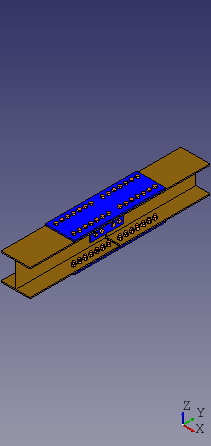
\includegraphics[width=\linewidth]{E:/office _anjali/columnspliceanjali/Osdag3/ResourceFiles/images/3d.png}%
\caption{3D View}%
\end{figure}

%
\end{document}